\section{Application to the Northern Provinces Household Nutrition Survey}
\label{sec:application}

\subsection{Data}
\label{sec:data}

The NPHNS was conducted between March and August 2021 by the provincial
statistical offices of the four northern provinces. It used a stratified
two-stage design in which enumeration areas were selected with probability
proportional to size within urban and rural strata of each province, and 12
households were selected systematically within each enumeration area. All
children aged 0--59 months in the selected households were eligible for
anthropometric measurement. The final sample comprised 9{,}412 children with
valid height-for-age measurements in 6{,}384 households, spread over the 214
districts of the four provinces. District sample sizes ranged from 7 to 163
children, with a median of 38.

Direct estimates of stunting prevalence were computed as H\'ajek-weighted
proportions. Because design-based variance estimates are themselves unstable in
districts with few sampled clusters, we smoothed them with a generalized
variance function, regressing the log of the estimated design effect on the log
of the district sample size and the number of sampled clusters, and setting
$\psi_i = \hat\theta_i^{\mathrm{syn}} (1 - \hat\theta_i^{\mathrm{syn}})\,
\hat d_i / n_i$, where $\hat\theta_i^{\mathrm{syn}}$ is a preliminary synthetic
estimate and $\hat d_i$ is the fitted design effect. The fitted design effects
ranged from 1.3 to 2.6.

The linear part of the model includes five district-level covariates taken from
the 2020 population census and administrative registers: the proportion of
households with an improved water source, the proportion of women aged 15--49
with completed secondary education, the proportion of households owning
livestock, the mean household size, and an indicator for districts that host a
provincial capital. The remoteness index $r_i$ was computed from a gridded
travel-time surface and district population grids; its median across districts
was 1.8 hours, with a maximum of 7.4 hours. As a secondary measure of access,
the mean distance from a household to the nearest health facility ranged from
2.1 to 38.5\,m across districts.

\subsection{Model fitting}

We fitted the FH, FH-log and SAFH models to the 214 district direct estimates.
The SAFH model used $K = 35$ knots. Table~\ref{tab:app} reports the estimated
variance components and summaries of the precision of the resulting district
estimates. Allowing a nonlinear effect of remoteness reduced the estimated
area-level variance from $\hat\sigma_u^2 = 0.0031$ under FH to
$\hat\sigma_u^2 = 0.0019$ under SAFH, indicating that a substantial part of the
between-district variation that the linear model attributes to unexplained
area effects is in fact explained by remoteness. A likelihood ratio test of
$H_0\colon \sigma_\gamma^2 = 0$, using the 50:50 mixture of $\chi^2_0$ and
$\chi^2_1$ distributions as the reference distribution
\citep{crainiceanu2004likelihood}, gave $p = 0.41$, so we reject the null
hypothesis of a linear remoteness effect.

The estimated function $\hat f$ increases steeply over the first two hours of
travel time and is nearly flat beyond four hours. Districts at a travel time of
four hours have an estimated prevalence about 9 percentage points higher than
otherwise similar districts at 30 minutes, whereas the FH model, constrained to
a straight line, implies a difference of only 5 percentage points over the same
range but overstates the difference for the few districts beyond six hours.

\begin{table}[t]
\centering
\caption{Estimated area-level variance and precision of the district estimates
under the three models, NPHNS 2021 ($m = 241$ districts). CV, coefficient of
variation.}
\label{tab:app}
\begin{tabular}{lrrr}
\toprule
 & FH & FH-log & SAFH \\
\midrule
$\hat\sigma_u^2$                    & 0.0031 & 0.0024 & 0.0019 \\
Median CV                           & 0.26   & 0.22   & 0.19   \\
Districts with CV $> 0.3$           & 61     & 38     & 23     \\
Districts with prevalence $> 25\%$  & 7      & 9      & 11     \\
\bottomrule
\end{tabular}
\end{table}

\subsection{District estimates}

The SAFH estimates are considerably more precise than the direct estimates, whose
median CV is 0.47, and also more precise than the FH estimates. The median CV of
the district estimates fell from 0.26 under FH to 0.19 under SAFH, a reduction
of 27\%, and the number of districts with a CV above 0.3, a threshold commonly
used by national statistical offices to decide whether an estimate can be
published, fell from 61 to 17. The gains are largest in the remote districts of
the two easternmost provinces, which have both the smallest samples and the
most extreme values of the remoteness index.

Figure~\ref{fig:map} maps the SAFH estimates. Under SAFH, eleven districts have
an estimated stunting prevalence above the national target of 25\%, compared
with seven under FH. All four additional districts lie in the eastern
highlands at travel times of two to four hours, where the FH model
underestimates prevalence because its linear remoteness term cannot follow the
curvature of $\hat f$. The national programme planned to prioritize districts above the target,
so the choice of model directly affects the allocation of the supplementary
feeding programme.

\begin{figure}[t]
\centering
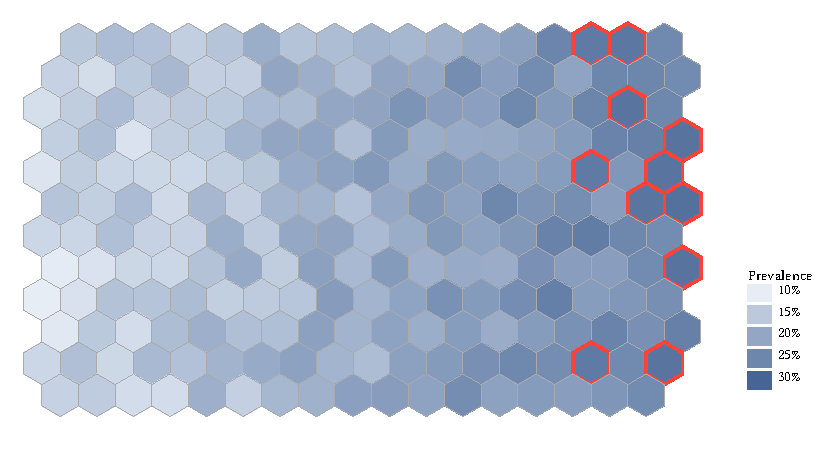
\includegraphics[width=0.8\textwidth]{figures/district_map.pdf}
\caption{SAFH estimates of stunting prevalence by district, NPHNS 2021.
Districts with an estimated prevalence above 25\% are outlined.}
\label{fig:map}
\end{figure}

As a design-based check, we compared the model-based estimates aggregated to the
provincial level with the direct provincial estimates, which are reliable at
that level. The SAFH estimates aggregated with census population weights
differed from the direct provincial estimates by at most 0.6 percentage points,
compared with up to 1.4 percentage points for FH, suggesting that the SAFH
estimates are well calibrated.
